%!TEX root = ../thesis_a4.tex

\chapter{Applications in Musicology}
\label{sec:musicology}

\section{Introduction}
\label{sec:musicology:introduction}

A vast amount of musical knowledge has been gathered for centuries by musicologists and music enthusiasts. Most of this knowledge is implicitly expressed in artist biographies, reviews, facsimile editions, etc. %Music Digital Libraries make this information available and searchable. 
%In addition, with the democratisation of Internet access, large amounts of music information generated by users is stored in online sources. 
This context results in the existence of large repositories of unstructured knowledge, which have great potential for musicological studies.
%Keyword-based search is generally provided either in the context of a Digital Library or a Web browser. However, implicit knowledge present in text is not fully understood by machines, so complex queries cannot be answered. 
For instance, aggregating musical and musicological information after processing large collections of naturally occurring text can provide search engines with much richer and fine-grained information about musicians, their life and work, and even their relation with other musical entities.

In this chapter we propose to explore two use cases where we reconcile, on one hand, intelligent text processing techniques, and on the other, musical knowledge acquired both from structured and unstructured resources. In the first use case, we create a culture-specific knowledge base, in particular, a knowledge base of flamenco music. The methodology applied to its creation combines content aggregation from different data sources and knowledge extraction. Then, a methodology for the creation of a knowledge graph from a set of unstructured text documents using entity linking is proposed and tested for computing artist relevance ranking. Evaluation shows a high level of agreement between a flamenco expert and our system.
In the second use case, we provide a diachronic study of music criticism via a quantitative analysis of the polarity associated to music album reviews gathered from \texttt{Amazon}\footnote{\url{http://www.amazon.com}}. Our analysis hints at a potential correlation between key cultural and geopolitical events and the language and evolving sentiments found in music reviews. In addition, trends observed in the data reveals to be useful to study the evolution of music genres.

%In this chapter we address the challenge of making sense of large amounts of unstructured texts in the context of musicological studies from two different perspectives. 
%(1) we propose a methodology for the creation of a culture-specific knowledge base; in particular, a knowledge base of flamenco music. The proposed methodology combines content aggregation from different data sources and a knowledge extraction process. Then, a methodology for the creation of a Knowledge Graph is proposed and tested for computing artist relevance ranking. Evaluation shows a high level of agreement between a flamenco expert and our system. %First, an important amount of information is gathered from different data sources, which are subsequently combined by applying pair-wise entity resolution. Next, new knowledge is extracted from unstructured harvested texts and employed to populate the knowledge base. For this purpose, an entity linking system has been expressly developed. 
%(2) 
%We present an analysis of the evolution of Music Digital Libraries from a technological perspective. In addition, a methodology to exploit implicit knowledge present in this kind of libraries is proposed and applied over a set of artist biographies gathered from the New Grove Dictionary. 
%(2) we provide a diachronic study of music criticism via a quantitative analysis of the polarity associated to music album reviews gathered from Amazon. Our analysis hints at a potential correlation between key cultural and geopolitical events and the language and evolving sentiments found in music reviews. In addition, trends observed in the data reveals to be useful to study the evolution of music genres.

The rest of the chapter is organized as follows. First, in Section~\ref{sec:musicology:flamenco-kb}, we describe the process of creation of a culture-specific knowledge base. We begin introducing the problem and the context of application. Then, we describe the obtained knowledge base and the processes of knowledge curation and extraction applied. Finally, we employ the knowledge base to compute artist relevance ranking and present some insights that can be drawn from computing statistics over the dataset. In Section~\ref{sec:musicology:evolution}, we describe how sentiment associated with music reviews changes over time. We start by describing the dataset of music reviews used and the process of aspect-based sentiment analysis applied. Then, two experiments are performed, one aggregating sentiment scores by review publication year, and other by album publication year. Finally, we conclude the chapter with a discussion about our findings (Section~\ref{sec:musicology:conclusions}). 


\section[Building culture-specific knowledge bases: the flamenco case][Building culture-specific KBs: the flamenco case]{Building culture-specific knowledge bases: the flamenco case}
\label{sec:musicology:flamenco-kb}

%Music context information is now playing a key role in MIR research. Multimodal approaches, semantic approaches, and text-IR approaches have shown important achievements in typical MIR problems, such as music recommendation and discovery, genre classification, or music similarity \citep{Schedl2014}. Therefore, collecting and storing music context information may be extremely useful for the MIR research community. 

Although some existing repositories of music information are quite complete and accurate, there is still a vast amount of music information out there, which is generally scattered across different sources on the Web. Hence, harvesting and combining that information is a crucial step in the creation of practical and meaningful music knowledge bases. In addition, the creation of culture-specific knowledge bases may be highly valuable for research and dissemination purposes, and can be particularly impactful in non-western traditions \citep{Serra2014compmusic}. 
%However, to the best of our knowledege, not many initiatives have been focused on this direction.

In this section, we propose a methodology for the creation of a culture-specific knowledge base; in particular, a knowledge base of flamenco music. The proposed methodology combines content curation and knowledge extraction processes. First, a large amount of information is gathered from different data sources, which are subsequently combined by applying pair-wise entity resolution. Next, new knowledge is extracted from unstructured texts and employed to populate the knowledge base. To this end, an \textit{ad hoc} entity linking system has been developed. Finally, the content of the knowledge base is used to compute artist relevance and results are evaluated according to flamenco experts criteria. %The content of the knowledge base is freely available and downloadable as data dumps in RDF and JSON formats.

%The remainder of the section is organized as follows. In Section~\ref{sec:musicology:flamenco}, an introduction to flamenco music is presented. In Section~\ref{sec:musicology:related_work}  some relevant prior work is briefly surveyed. Section~\ref{sec:musicology:flabase} describes the structure of the knowledge base. Next, in Section~\ref{sec:musicology:kb_curation} the process of content curation is explained. Section~\ref{sec:musicology:kb_extraction} shows the methodology applied for knowledge extraction. In Section~\ref{sec:musicology:statistics} artist relevance is computed and some statistics about the content are laid out. Finally, Section~\ref{sec:musicology:conclusion} concludes the paper and points out for future lines of work.

\subsection{Flamenco music}
\label{sec:musicology:flamenco}

Several musical traditions contributed to the genesis of flamenco music as we know it today. Among them, the influences of the Jews, Arabs, and Spanish folk music are recognizable, but indubitably  the imprint of Andalusian Gypsies' culture is deeply ingrained in flamenco music. 
Flamenco occurs in a wide range of settings, including festive \textit{juergas} (private parties), \textit{tablaos} (flamenco venues), concerts, and big productions in theaters. In all these settings we find the main components of flamenco music: \textit{cante} or singing, \textit{toque} or guitar playing, and \textit{baile} or dance. According to \cite{gamboa-05}, flamenco music grew out of the singing tradition, as a melting process of all the traditions mentioned above, and therefore the role of the singer soon became dominant and fundamental. \textit{Toque}  is subordinated to \textit{cante}, especially in more traditional settings, whereas \textit{baile} enjoys more independence from voice. 

In the flamenco jargon styles are called \textit{palos}. Criteria adopted to define flamenco \textit{palos} are rhythmic patterns, chord progressions, lyrics and its poetic structure, and geographical origin. In flamenco geographical variation is important to classify \textit{cantes} as often they are associated to a particular region where they were originated or where they are performed with gusto. 
Rhythm or \textit{comp\'as} is a unique feature of flamenco.
Rhythmic patterns based on 12-beat cycles are mainly used. Those patterns can be classed as follows: binary patterns, such as \textit{tangos} or \textit{tientos}; ternary patterns, which are the most common ones, such as \textit{fandangos} or \textit{buler\'ias}; mixed patterns, where ternary and binary patterns alternate, such as \textit{guajira}; free-form, where there is no a clear underlying rhythm, such as \textit{ton\'as}.
For further information on fundamental aspects of flamenco music, see the book of Fern\'andez~\citep{fer-04}. For a comprehensive study of styles, musical forms and history of flamenco the reader is referred to the books of Blas Vega and R\'ios Ruiz~\citep{bvrr-88}, Navarro and Ropero~\citep{nr-95}, and Gamboa~\citep{gamboa-05} and the references therein.


\subsection{FlaBase}
\label{sec:musicology:flabase}

FlaBase (Flamenco Knowledge Base) is the acronym of a new knowledge base of flamenco music. Its ultimate aim is to gather all available online editorial, biographical and musicological information related to flamenco music. Its content is the result of the curation and extraction processes explained in Sections \ref{sec:musicology:kb_curation} and \ref{sec:musicology:kb_extraction}. %FlaBase is stored in RDF and JSON formats, and it is freely available for download\footnote{\url{http://mtg.upf.edu/download/datasets/flabase}}. Its RDF version follows the Linked Open Data principles, and it might be queried by setting up a SPARQL endpoint. A JSON version is also available, thus facilitating the use of the content by all the community of researchers and developers. 
FlaBase contains information about 1,174 artists, 76 \textit{palos} (flamenco genres), 2,913 albums, 14,078 tracks, and 771 Andalusian locations.

%Every entity in FlaBase is viewed as a resource, and every resource is classified by the FlaBase ontology.To define the properties of different classes of resources an initial ontology have been defined. In what follows, the ontology schema is shown and some statistics of the content available in Flabase are summarized.

\subsubsection{Ontology definition}
\label{sec:musicology:ontology}

The FlaBase data structure is defined following an ontology schema. One of the advantages of using an ontology is that it can be easily modified. Thus, our design is a first building block that can be enhanced and redefined in the future. The initial ontology is structured around five main classes: MusicArtist, Album, Track, Palo and Place, and three domain specific classes: \textit{cantaor} (flamenco singer), guitarist (flamenco guitar player), and \textit{bailaor} (flamenco dancer). These three classes were defined because they are the most frequent types of artists in the data. Other instrument players may be instantiated directly from the MusicArtist class. 
%A diagram with the main classes and some properties of the ontology is shown in Figure~\ref{fig:musicology:ontology}.
%We are aware of other music standard schemas such as the Music Ontology \footnote{\url{http://musicontology.com/}}, however, we opted to define our own ontology in order to let the schema as simple as possible. By the way, class and property equivalence has been defined through the OWL\footnote{\url{http://www.w3.org/TR/owl2-overview/}} properties owl:equivalentClass and owl: equivalentProperty between our classes and properties and those from the Music Ontology (e.g. MusicArtist, Track, Genre).
We have tried to reuse as much vocabulary as we could. We re-utilized most of the classes and some properties from the Music Ontology\footnote{\url{http://musicontology.com}}, a standard model for publishing music-related data. We selected the classes according to the ones used by the LinkedBrainz project\footnote{\url{https://wiki.musicbrainz.org/LinkedBrainz}}, which maps concepts from MusicBrainz to Music Ontology.

\iffalse
\begin{figure}
	\centering
	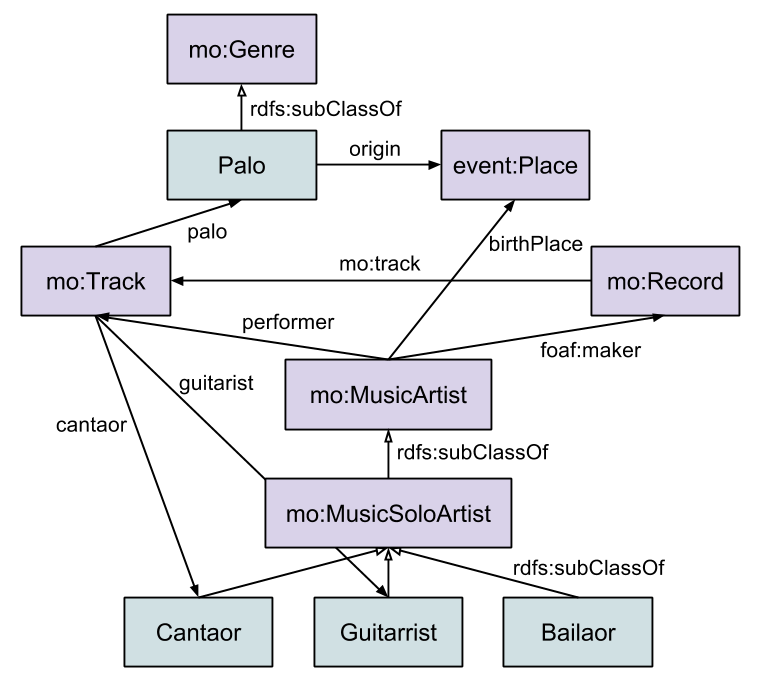
\includegraphics[width=0.40\textwidth]{ch05_musicology_pics/flabase_ontology2.png}
	\caption{Ontology schema \label{fig:musicology:ontology}}
\end{figure}
\fi


\subsection{Content curation}
\label{sec:musicology:kb_curation}

The first step towards building a domain-specific knowledge base is to gather all possible content from available data sources. This implies at least two problems, namely, the selection of sources, and the matching between entities from different sources (entity resolution). In what follows we enumerate the involved data sources and describe the methodology applied for entity resolution.

\subsubsection{Data acquisition}
\label{sec:musicology:datasoruces}

Our aim is to gather an important amount of information about musical entities, including textual descriptions and available metadata. A schema of the selected data sources is shown in Figure~\ref{fig:musicology:datasources}. We started by looking at Wikipedia.%, the free and multilingual Internet encyclopedia. It is the Internet's largest and most popular general reference work. 
Each Wikipedia article may have a set of associated categories. Categories are intended to group together pages on similar subjects and are structured in a taxonomical way. To find Wikipedia articles related to flamenco music, we first looked for flamenco categories. The taxonomy of categories can be explored by querying DBpedia. %, a knowledge base with structured content extracted from Wikipedia. 
In particular, we employed the SPARQL endpoint of the Spanish DBpedia\footnote{\url{http://es.dbpedia.org}}. We queried for categories related to the flamenco category in the taxonomy. At the end, we obtained 17 different categories (e.g., \textit{cantaores de flamenco, guitarristas de flamenco}).

\begin{figure}
	\centering
	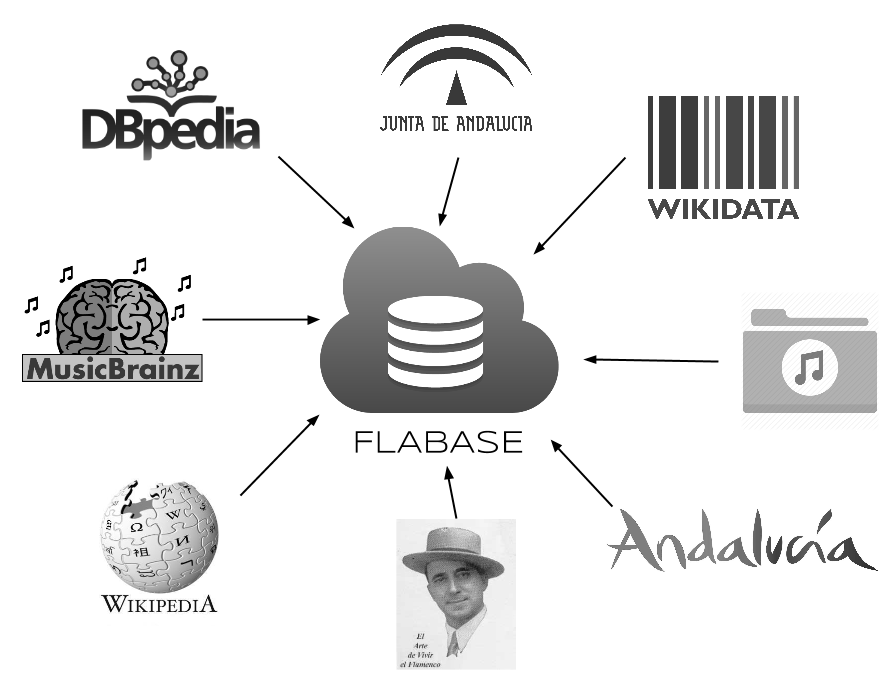
\includegraphics[width=0.55\textwidth]{ch05_musicology_pics/datasources_bn.png}
	\caption{Selected data sources \label{fig:musicology:datasources}}
\end{figure}

%DBpedia resources are related to categories through the property dcterms:subject. Thus, b
By querying again DBpedia, we gathered all DBpedia resources related to one of these categories. We obtained a total number of 438 resources in Spanish, of which 281 were also in English. Each DBpedia resource is associated with a Wikipedia article. Text and HTML code were then extracted from Wikipedia articles in English and Spanish by using the WikiMedia API. 
%From DBpedia, we also gathered some biographical structured information of each resource, when it was available. 
Next, we classified the extracted articles according to our ontology (Section~\ref{sec:musicology:ontology}). For this purpose, we exploited classification information provided by DBpedia (DBpedia types and Wikipedia categories). At the end, from all gathered resources, we only kept those related to artists and \textit{palos}, totaling  291 artists and 56 \textit{palos}.

As the amount of information present in Wikipedia related to flamenco music is somewhat scarce, we decided to expand our knowledge base with information from two different websites. First, \textit{Andalucia.org}, the touristic web from the Andalusia Government\footnote{\url{http://andalucia.org}}. It contains 422 artist biographies in English and Spanish, and the description of 76 \textit{palos} also in both languages. Second, a website called \textit{El arte de vivir el flamenco}\footnote{\url{http://www.elartedevivirelflamenco.com/}}, which includes 749 artist biographies among \textit{cantaores}, \textit{bailaores} and guitarists. Both webs were crawled and their content stored in our knowledge base. %As it is explained in Section~\ref{sec:musicology:entity_resolution}, artists from the three datasources were mapped, obtaining a final set of 1,176 different artists.

%MusicBrainz is one of the biggest and more reliable open music databases, which provides an unambiguous form of music identification. Therefore, we turned to it 
We used MusicBrainz to fill our knowledge base with information about flamenco album releases and recordings. Artists present in FlaBase were intended to be mapped with MusicBrainz artists. For every match, all content related to releases and recordings was gathered. After doing so, we obtained a total number of 814 releases and 9,942 recordings. 
%AcousticBrainz\footnote{\url{http://acousticbrainz.org}} is a project that aims to crowd source acoustic information for all music tracks identified in MusicBrainz. We queried the AcousticBrainz API for the acoustic descriptors of MusicBrainz recordings. We found acoustic information of 620 of the stored recordings.%, and kept it in our knowledge base.

The information gathered from MusicBrainz is a little part of the actual flamenco discography. Therefore, to complement it we used a flamenco recordings database gathered by Rafael Infante and available at CICA website\footnote{\url{http://flun.cica.es/index.php/grabaciones}} (Computing and Scientific Center of Andalusia). This database has information about releases from the early time of recordings until present time, counting 2,099 releases and 4,136 songs. For every song entry, a \textit{cantaor} name is provided, and most of the times also guitarist and \textit{palo}, which is an important piece of information to define flamenco recordings.

Finally, we supplied our knowledge base with information related to Andalusian towns and provinces. We gathered this information from the official database SIMA\footnote{\url{http://www.juntadeandalucia.es/institutodeestadisticaycartografia/sima}} (Multi-territorial System of Information of Andalusia).%, of the Official Institute of Statistics and Cartography of Andalusia. 


\subsubsection{Entity resolution}
\label{sec:musicology:entity_resolution}

Entity resolution is the problem of extracting, matching and resolving entity mentions in structured and unstructured data \citep{Getoor2012}. There are several approaches to tackle the entity resolution problem. For the scope of this research, we selected a pair-wise classification approach based on string similarity between entity labels.

The first issue after gathering the data is to decide whether two entities from different sources are referring to the same one. Therefore, given two sets of entities $A$ and $B$, the objective is to define an injective and non-surjective mapping function $f$ between $A$ and $B$ that decides whether an entity $a \in A$ is the same as an entity $b \in B$. To do that, a string similarity metric $sim(a,b)$ based on the Ratcliff-Obershelp algorithm \citep{Ratcliff1988} has been defined. It measures the similarity between two entity labels and outputs a value between 0 and 1. We consider that $a$ and $b$ are the same entity if their similarity is bigger than a parameter $\theta$. If there are two entities $b, c \in B$ that satisfy that $sim(a,b) \geq \theta$ and $sim(a,c) \geq \theta$, we consider only the mapping with the highest score. To determine the value of $\theta$, we tested the method with several $\theta$ values over an annotated dataset of entity pairs. To create this dataset, the 291 artists gathered from Wikipedia were manually mapped to the 422 artists gathered from Andalucia.org, obtaining a total amount of 120 pair matches. As it is shown in Figure~\ref{fig:musicology:fmeasure} the best F-measure (0,97) was obtained with $\theta=0.9$. Finally, we applied the described method with $\theta=0.9$ to all gathered entities from the three data sources. Thanks to the entity resolution process, we reduced the initial set of 1,462 artists and 132 \textit{palos} to a set of 1,174 artists and 76 \textit{palos}.

\begin{figure}
	\centering
	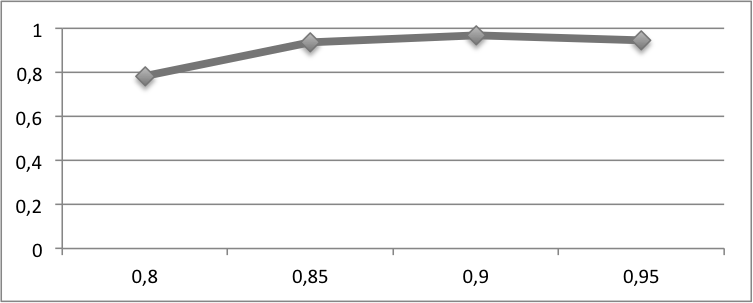
\includegraphics[width=0.60\textwidth]{ch05_musicology_pics/similarity_f_bn.png}
	\caption{F-measure for different values of $\theta$ \label{fig:musicology:fmeasure}}
\end{figure}

Once we had our artist entities resolved, we began to gather their related discographic information. First, we tried to find out the MusicBrainz ID of the gathered artists. Depending on the information about the entity, two different process were applied. First, every Wikipedia page has a correspondent entity defined in Wikidata\footnote{\url{https://www.wikidata.org}}. Wikidata is a free linked database which acts as a structured data storage of Wikipedia. There are several properties in Wikidata that may link Wikidata items with MusicBrainz items. %Thus, the equivalent Wikidata resource of a Wikipedia artist page may have a link to its corresponding MusicBrainz artist ID. 
We looked for these relations and mapped all possible entities. For those artists without a direct link to MusicBrainz, we queried the MusicBrainz API by using the artists names, and then applied our entity resolution method to the obtained results.

Finally, to integrate the discography database of CICA into our knowledge base, we applied the entity resolution method to the fields \textit{cantaor}, guitarist and \textit{palo} of each recording entry in the database. From the set of 202 \textit{cantaores} and 157 guitarists names present in the recording entries of the database, a total number of 78 \textit{cantaores} and 44 guitarists were mapped to our knowledge base. The number of mapped artists was low due to differences between the way of labeling an artist. An artist name may be written using one or two surnames, or using a nickname. In the case of \textit{palos}, there were 162 different \textit{palos} in the database, 54 of which were mapped with the 76 of our knowledge base. These 54 \textit{palos} correspond to an 80\% of \textit{palo} assignments present in the recording entries.


\subsection{Knowledge extraction}
\label{sec:musicology:kb_extraction}

While the resulting knowlege base does already encode relevant culture and music-specific information, a notable portion of the data collected during the knowledge base creation process currently remains unexploited due to its unstructured nature. In fact, the huge epistemic potential of free text in this version of the knowledge base has not still been harnessed. Consequently, to enhance the amount of structured data in FlaBase, a process of knowledge extraction has been carried out. This implicit knowledge may vary from biographical data, such as place and date of birth, to more complex semantic relations involving different entities. Three tasks play a key role in the process of knowledge extraction from non-structured text: named entity recognition (NER), entity linking (EL), and relation extraction \citep{Usbeck2014}. In this section, we focus on the two first tasks. In what follows, our \textit{ad hoc} system for entity recognition and disambiguation is described and evaluated. Lastly, an information extraction process is applied to populate the knowledge base.

\subsubsection{Named entity recognition and disambiguation}\label{sec:musicology:entity_linking}

In order to extract knowledge from a text, the first step is to semantically annotate it identifying all entity mentions. %Named entity recognition is a task that seeks and classify words in text into pre-defined categories (e.g., person, organization, or place). Named entity disambiguation, also called entity linking, aims to determine what is actually a named entity present in a text. It generally does so by identifying it in a knowledge base of reference. 
Entity linking can be addressed directly from the text, or applied to the output of a NER system. We propose a method that employs a combination of both approaches, depending on the category of the entity. For NER, we used the Stanford NER system \citep{Finkel2005}, implemented in the library Stanford Core NLP\footnote{\url{http://nlp.stanford.edu/software/corenlp.shtml}} and trained on Spanish texts. For EL we applied two different approaches. First, we looked for exact string matches between FlaBase entity labels and word n-grams extracted from the text. Second, we searched for exact string matches between FlaBase entity labels and named entities identified of the NER system. We tried several combinations of both approaches until we obtained the most satisfactory one.

%We selected all biography texts in Spanish from artists present in our knowledge base. 
For the scope of this research, we focused on Spanish texts, as flamenco texts are mostly written in Spanish. Although there are many entity linking tools available, state-of-the-art systems are well-tuned for English texts, but may not perform as well in languages other than English, and even less with music related texts (see Section~\ref{sec:linking:el}). In addition, we wanted to have a system that uses our own knowledge base. Therefore, we developed our own system, which is able to detect and disambiguate three categories of entities: person, \textit{palo} and location. Three different approaches were defined by combining NER and EL in different ways. First, directly applying EL to text. Second, disambiguating location and person entities from the NER output, and \textit{palo} directly from text. Third, only disambiguating location entities from the NER output, and location and \textit{palo} directly from text.

To determine which approach performs better, three artist biographies coming from three different data sources were manually annotated, having a total number of 49 annotated entities. We followed an evaluation methodology similar to the one used in KBP2014 Entity Linking Task\footnote{\url{http://nlp.cs.rpi.edu/kbp/2014/}}. Results on the different approaches are shown in Table~\ref{tbl:musicology:res1}. We observe that applying NER to entities of the person category before EL worsens performance significantly, as recall suddenly decreases by half. After manually analyzing false negatives, we observed that this is caused because many artist names have definite articles between name and surname (e.g., \textit{de, del}), and this is not recognized by the NER system. In addition, many artists have a nickname that is not interpreted as a person entity by the NER system. The best approach is the third (EL + NER to LOC), which is slightly better than the first (only EL) in terms of precision. This is due to the fact that many artists have a town name as a surname or as part of his nickname. Therefore, applying EL directly to text is misclassifying person entities as location entities. Thus, by adding a previous step of NER to location entities we have increased overall performance, as it can be seen on the F-measure values.

\begin{table}
	\centering
%\begin{adjustbox}{max width=8cm}
	  \begin{tabular}{  l c c c }
    \hline
    Approach & Precision & Recall & F-measure \\ 
    \hline
    1) EL & 0.829 & \textbf{0.694} & 0.756 \\ 
    2) EL + NER to PERS \& LOC & 0.739 & 0.347 & 0.472 \\
    3) EL + NER to LOC & \textbf{0.892} & 0.674 & \textbf{0.767} \\
    \hline
  \end{tabular}
%  \end{adjustbox}
	\caption{Precision, Recall and F-measure of NER+EL}
	
	\label{tbl:musicology:res1}
\end{table}

\subsubsection{Knowledge base population}
\label{sec:musicology:ie}

Biographical texts coming from different data sources have been stored in FlaBase. These texts are full of relevant information about FlaBase entities, but in an unstructured way. Thus, a process of information extraction is necessary to transform the unstructured information into structured knowledge. For the scope of this research, we focused on extracting two specific pieces of information: birth year and birth place, as they can be relevant for anthropological studies. We observed that this information is often in the first sentences of the artist biographies, and always near the word \textit{naci\'{o}} (Spanish translation of ``was born"). Therefore, to extract this information, we looked for this word in the first 250 characters of every biographical text. If it is found, we apply our entity linking method to this piece of text. If a location entity is found near the word "naci\'{o}", we assume that this entity is the place of birth of the biography subject. In addition, by using regular expressions, we look for the presence of a year expression in the neighborhood. If it is found, we assume it as the year of birth. If more than one year is found, we select the one with the smaller value. 

To evaluate our approach, we tested the extraction of birth places in all texts coming from the web Andalucia.org (442 artists). %We chose this subset because Andalucia.org also provides specific information about artist origin that had been previously crawled and stored in FlaBase. However, we observed that in many occasions the artist origin provided by the data source was wrong. Therefore, we decided to 
We manually annotated the province of provenance of these 442 artists for building ground truth data. After the application of the extraction process on the annotated test set, we obtained a precision value of 0,922 and a recall of 0,648. Therefore, we may argue that our method is extracting biographic information with high precision and quite reasonable recall. 
%In addition, the information extracted by our system is indeed more accurate than the actual information provided by the data source. 
We finally applied the extraction process to all artist entities with biographical texts coming from any of the two flamenco crawled websites. Thus, %from a total number of 1,123 artists coming from these data sources (95\% of the artists in the knowledge base), 
743 birth places and 879 birth years were extracted. 

\subsection{Looking at the data}
\label{sec:musicology:data-analysis}

\subsubsection{Artist relevance}
\label{sec:musicology:relevance}

We assume that an entity mention inside an artist biography signals a semantic relation between the entity that constitutes the main theme of the biography (subject entity) and the mentioned entity. Based on this assumption, we build a semantic graph by applying the following steps. First, each artist of the knowledge base is added to the graph as a node. Second, entity linking is applied to artist's biographical texts. For every linked entity identified in the biography, a new node is created in the graph (only if it was not previously created). Next, an edge is added, connecting the subject entity with the linked entity found in its biography. This way, a directed graph connecting the entities of FlaBase is finally obtained. Entities identified in a text can be seen as hyperlinks. Thus, algorithms to measure the relevance of nodes in a network of hyperlinks can be applied to our semantic graph \citep{Bellomi2005}. In order to measure artist relevance, we applied PageRank \citep{Brin1998} and HITS \citep{Kleinberg1999} algorithms to the obtained graph. 
%PageRank outputs a measure of relevance for each node, and HITS gives two different results: \textit{authority} and \textit{hubness}. We only take into consideration \textit{authority} from HITS algorithm, because it is proven to be the most effective of both values as a relevancy metric \citep{Bellomi2005}.

Using this approach, we built an ordered list with the top-10 entities of the different artist categories (\textit{cantaor}, guitarist and \textit{bailaor}) for the two algorithms. For evaluation purposes, we asked a reputed flamenco expert to build a list of top-10 artists for each category according to his knowledge and the available bibliography. The concept of artist relevance is somehow subjective and there is no unified or consensual criteria for flamenco experts about who the most relevant artists are. Despite that, there is a high level of agreement among them on certain artists that should be on such a hypothetical list. Thus, the expert provided us with this list of hypothetical top-10 artists by category and we considered it as ground truth. We define precision as the number of identified artists in the resulting list that are also present in the ground truth list divided by the length of the list. We evaluated the output of the two algorithms by calculating precision over the entire list (top-10), and over the first five elements (top-5) (see Table~\ref{tbl:musicology:experts_results}). We can observe that Page\-Rank results (see Table~\ref{tbl:musicology:pagerank}) show the greatest agreement with the flamenco expert. 
High values of precision, especially for the top-5 list, indicates that the content gathered in FlaBase is highly complete and accurate (see Table~\ref{tbl:musicology:experts_results}), and the proposed methodology adequate to compute relevance of artists. 

\inputencoding{latin1}
\begin{table}[]
    \centering
%\begin{adjustbox}{max width=8cm}
    \begin{tabular}{c c c }
    \hline
    \textit{Cantaor} & Guitarist & \textit{Bailaor} \\
    \hline
Antonio Mairena & Paco de Luc\'{i}a & Antonio Ruiz Soler \\
Manolo Caracol & Ram\'{o}n Montoya & Rosario \\
La Ni\~{n}a de los Peines & Ni\~{n}o Ricardo & Antonio Gades \\
Antonio Chac\'{o}n & Manolo Sanl\'{u}car & Mario Maya \\
Camar\'{o}n de la Isla & Sabicas & Carmen Amaya \\
%Manuel Torre & Tomatito & Pilar López \\
%José Mercé & Vicente Amigo & La Argentinita \\
%Enrique Morente & Gerardo Núñez & Lola Flores \\
%Pepe Marchena & Paco Cepero & Pastora Imperio \\
%Manuel Vallejo & Pepe Habichuela & José Antonio \\
    \hline
    \end{tabular}
%   \end{adjustbox}
    \caption{PageRank Top-5 artists by category.}    
    \label{tbl:musicology:pagerank}
\end{table}
\inputencoding{utf8}

%Among the different categories, the list of \textit{cantaores} exhibit the best agreement with the ground truth. This is probably due to the fact that there is more information about this particular category in FlaBase (47\% of \textit{cantaores}, 29\% of guitarists, and 22\% of \textit{bailaores)}. 
%As it is shown in Figure~\ref{fig:musicology:graph-type}, the amount of cantaores is substantially higher than the other two categories.


\begin{table}[]
    \centering
%\begin{adjustbox}{max width=8cm}
    \begin{tabular}{ c c c }
    \hline
    & Top-5 & Top-10 \\
    \hline
    PageRank & 0.933 & 0.633 \\
    HITS Authority & 0.6 & 0.4 \\
    \hline
    \end{tabular}
%   \end{adjustbox}
    \caption{Precision values of artist relevance ranking.}    
    \label{tbl:musicology:experts_results}
\end{table}

\subsubsection{Statistics}
\label{sec:musicology:statistics}

For the sake of completeness, we computed the distribution of different items present in FlaBase. 
% after the processes of curation and extraction.  
Data shown in Figure~\ref{fig:musicology:graph-palo} was produced after the knowledge acquisition process, while data shown in Figures \ref{fig:musicology:graph-province} and \ref{fig:musicology:graph-decade} was obtained thanks to the knowledge extraction process. In Figure~\ref{fig:musicology:graph-palo} it is shown that the most representative \textit{palos} in flamenco music are represented in our knowledge base, with a higher predominance of fandangos. We can observe in Figure~\ref{fig:musicology:graph-province} that most flamenco artists are from the Andalusian provinces of Seville and Cadiz. 
Finally, in Figure~\ref{fig:musicology:graph-decade} we observe a higher number of artists in the data were born from the 30's to the 80's of the 20th century.

%\begin{figure}
%    \centering
%    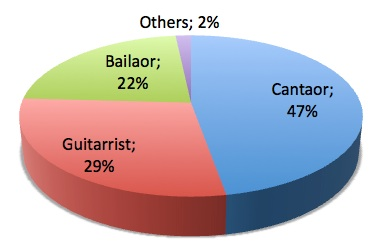
\includegraphics[width=6cm]{figs/Artists-by-type.jpg}
%    \caption{Artists by type 
%    \label{fig:musicology:graph-type}}
%\end{figure}

\begin{figure}[ht!]
    \centering
    \begin{subfigure}{.45\textwidth}
        \centering
        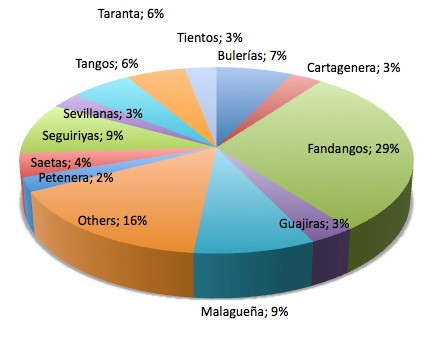
\includegraphics[width=.9\linewidth]{ch05_musicology_pics/Songs-by-palo.jpg}
    	\caption{Songs by \textit{palo}}
        \label{fig:musicology:graph-palo}
    \end{subfigure}
    \begin{subfigure}{.52\textwidth}
        \centering
        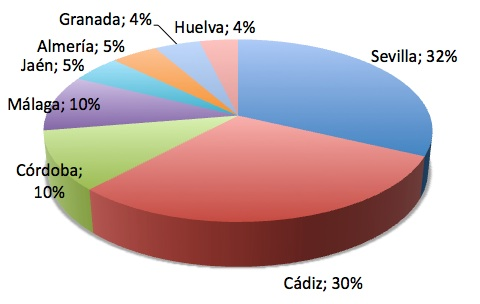
\includegraphics[width=.9\linewidth]{ch05_musicology_pics/Artists-by-province.jpg}
		\caption{Artists by province of birth}
		\label{fig:musicology:graph-province}
    \end{subfigure}
    \caption{FlaBase distributions.}
\end{figure}


\begin{figure}[!ht]
	\centering
	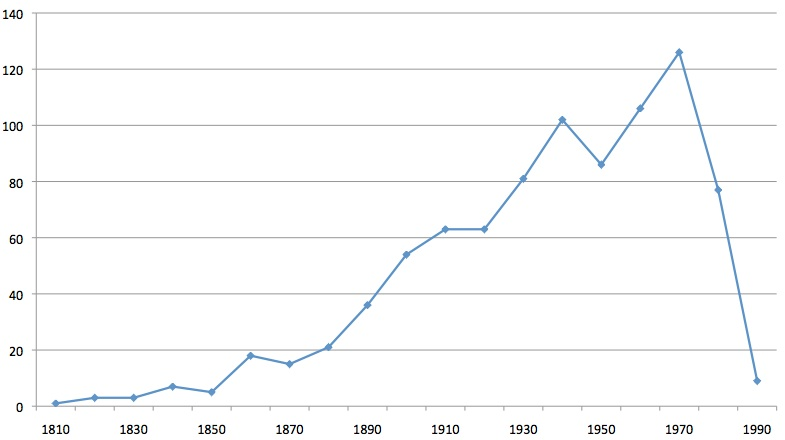
\includegraphics[width=8cm]{ch05_musicology_pics/Artists-by-decade-of-birth.jpg}
	\caption{Artists by decade of birth 
	\label{fig:musicology:graph-decade}}
\end{figure}


\section{Diachronic study of music criticism}
\label{sec:musicology:evolution}

In this Section, we put forward an integration procedure for enriching a large corpus of Amazon customer reviews \citep{McAuley2015a,McAuley2015}, with metadata obtained from MusicBrainz\footnote{\url{http://musicbrainz.org/}}. %AcousticBrainz (AB) is a database of music and audio descriptors, computed from audio recordings via state-of-the-art Music Information Retrieval algorithms \citep{Porter2015}.
In addition, we further extend the \textit{semantics} of the textual content with the application of an aspect-based sentiment analysis framework \citep{DongSOS13} which provides specific sentiment scores for different aspects present in the text, e.g. album cover, guitar, voice or lyrics.

This enriched dataset, henceforth referred to as Multimodal Album Reviews Dataset (MARD), includes affective features and music metadata. % such as album release date.
We benefit from this substantial amount of information at our disposal for performing a diachronic analysis of music criticism. Specifically, we combine the metadata retrieved for each review with their associated sentiment information, and generate visualizations to help us investigate any potential trends in diachronic music appreciation and criticism. Based on this evidence, and since music evokes emotions through mechanisms that are not unique to music \citep{Juslin2008}, we may go as far as using musical information as means for a better understanding of global affairs. Previous studies argue that national confidence may be expressed in any form of art, including music \citep{Moisi2010}, and in fact, there is strong evidence suggesting that our emotional reactions to music have important and far-reaching implications for our beliefs, goals and actions, as members of social and cultural groups \citep{Alcorta2008}. Our analysis hints at a potential correlation between the language used in music reviews and major geopolitical events or economic fluctuations. Finally, we argue that applying sentiment analysis to music corpora may be useful for diachronic musicological studies.


\subsection{Dataset}
\label{sec:musicology:mard}

The collected dataset contains texts and accompanying metadata originally obtained from a much larger dataset of Amazon customer reviews \citep{McAuley2015a,McAuley2015}. The original dataset provides millions of review texts together with additional information such as overall rating (between 0 to 5), date of publication, or creator id. Each review is associated to a product and, for each product, additional metadata is also provided, namely Amazon product id, list of similar products, price, sell rank and genre categories. From this initial dataset, we selected the subset of products categorized as \textit{CDs \& Vinyls}, which also fulfill the following criteria. First, considering that the Amazon taxonomy of music genres contains 27 labels in the first hierarchy level, and about 500 in total, we obtain a music-relevant subset and select 16 of the 27 which really define a music style and discard for instance region categories (e.g. World Music) and other categories non specifically related to a music style (e.g. Soundtrack, Miscellaneous, Special Interest), function-oriented categories (Karaoke, Holiday \& Wedding) or categories whose albums might also be found under other categories (e.g. Opera \& Classical Vocal, Broadway \& Vocalists). We compiled albums belonging only to one of the 16 selected categories, i.e. no multi-label. Note that the original dataset contains not only reviews about CDs and Vinyls, but also about music DVDs and VHSs. Since these are not strictly speaking music audio products, we filter out those products also classified as "Movies \& TV". Finally, since products classified as Classical and Pop are substantially more frequent in the original dataset, we compensate this unbalance by limiting the number of albums of any genre to 10,000. After this preprocessing, MARD amounts to a total of 65,566 albums and 263,525 customer reviews. A breakdown of the number of albums per genre is provided in Table~\ref{tbl:musicology:dataset}.

%This dataset is formed by texts and metadata coming from Amazon costumers reviews from the "CDs \& Vinyls" section. It is a subset of a large dataset of costumer reviews gathered in \cite{McAuley2015a,Mauch150081}. Review texts come with some extra information , i.e. overall rating, date of publication and creator id. Every review is related to a music album. For every album there is also some attached information, i.e. title, Amazon product id, list of similar products, price, sell rank and genre categories. From the initial dataset, we selected those products that fulfill the following criteria. The Amazon taxonomy of genres has 27 genres in the first hierarchy level, and more than 500 in total. From the 27 categories, we selected 16 define a music style, and not a region (e.g. Asian music) or another classification criteria (e.g. Soundtrack). We selected albums that are classified into only one of 16 selected categories. The original dataset has not only reviews about CDs and Vinyls, but also music DVDs and VHSs. Hence, to focus only on audio products, we filter out products that were also categorized as "Movies \& TV" or were ranked in the Video sales ranking. In the original dataset, there is a higher predominance of products classified as Classical and Pop. To compensate that, we limited the number of albums of these genres to 10,000 in the final dataset. After the filtering process we kept a total of 65,566 albums and 263,525 customer reviews, which comprises the core of our dataset. The amount of albums by genre is shown in Table~\ref{tbl:musicology:dataset}.

\begin{table}[h]
\scriptsize
\centering
\begin{tabular}{l r r r}
\hline
\textbf{Genre} & \textbf{Amazon} & \textbf{MusicBrainz} \\%& \textbf{AcousticBrainz} \\
\hline
Alternative Rock & 2,674 & 1,696 \\%& 564 \\
Reggae & 509 & 260 \\%& 79 \\
Classical & 10,000 & 2,197 \\%& 587 \\
R\&B & 2,114 & 2,950 \\%& 982 \\
Country & 2,771 & 1,032 \\%& 424 \\
Jazz & 6,890 & 2,990 \\%& 863 \\
Metal & 1,785 & 1,294 \\%& 500 \\
Pop & 10,000 & 4,422 \\%& 1701 \\
New Age & 2,656 & 638 \\%& 155 \\
Dance \& Electronic & 5,106 & 899 \\%& 367 \\
Rap \& Hip-Hop & 1,679 & 768 \\%& 207 \\
Latin Music & 7,924 & 3,237 \\%& 425 \\
Rock & 7,315 & 4,100 \\%& 1482 \\
Gospel & 900 & 274 \\%& 33 \\
Blues & 1,158 & 448 \\%& 135 \\
Folk & 2,085 & 848 \\%& 179 \\
\hline
\textbf{Total} & 66,566 & 28,053 \\%& 8,683 \\
\hline
\end{tabular}
\caption{Number of albums by genre with information from the different sources in MARD.}
\label{tbl:musicology:dataset}
\end{table}

Having performed genre filtering, we enrich MARD by extracting artist names and record labels from the Amazon product page. We pivot over this information to query the MusicBrainz search API to gather additional metadata such as release id, first release date, song titles and song ids. Mapping with MusicBrainz is performed using the same methodology described in Section~\ref{sec:musicology:entity_resolution}, following a pair-wise entity resolution approach based on string similarity with a threshold value of $\theta=0.85$. We successfully mapped 28,053 albums to MusicBrainz. %Then, we retrieved songs' audio descriptors from AB. From the 28,053 albums mapped to MusicBrainz, a total of 8,683 albums are further linked to their corresponding AB entry, which encompasses 65,786 songs. The final dataset is freely available for download\footnote{http://mtg.upf.edu/download/datasets/mard}.


%Note that this is the number of songs present in AB at the time of the dataset creation, however, AB is continuously growing and more albums from the total mapped to MB might be also found in the future in AB. 

%A summary of the properties of our dataset and the interplay of the three resources is shown in Figure \ref{fig:musicology:dataset}, using the album ``The Adventures of Rick Slick'' (Rick Slick) as an example.

%\begin{figure}[!h]
%  \centering
%	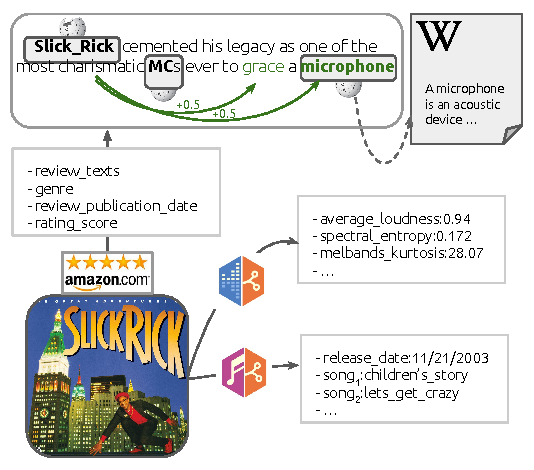
\includegraphics[width=8cm,height=7.25cm]{figs/dataset}
%  \caption{Summary of enrichment for every album review in our dataset, containing ontological (MB) and acoustic (AB) information as well as textual semantics.}
%  \label{fig:musicology:dataset}
%\end{figure}

%Once this genre-wise filtering was performed, we enrich the original ADR with artist name and record label. retrieved some extra information from Amazon that was not included in the original dataset, i.e. artist name and record label. Using the artist name and the album title we queried the MusicBrainz search API to try to gather more metadata about the albums, i.e. release group MBID (MusicBrainz ID), first release date, song titles and song MBID. For the mapping with MusicBrainz we followed a methodology similar to the one described in \cite{Flabase}. From the filtered set of albums, we obtained a mapping with MusicBrainz of 28,053 albums. Having the  MBIDs of the album songs, we can retrieve their audio descriptors present in AcousticBrainz. AcousticBrainz is a database of music descriptors computed from audio recordings using a number of state-of-the-art Music Information Retrieval algorithms. From the albums mapped to MusicBrainz, we found 8,683 albums for which their song descriptors were stored in AcousticBrainz. Audio descriptors of a total number of 65,786 songs were retrieved from AcousticBrainz.


\subsection{Sentiment analysis}
\label{sec:musicology:sentiment}

\begin{figure}
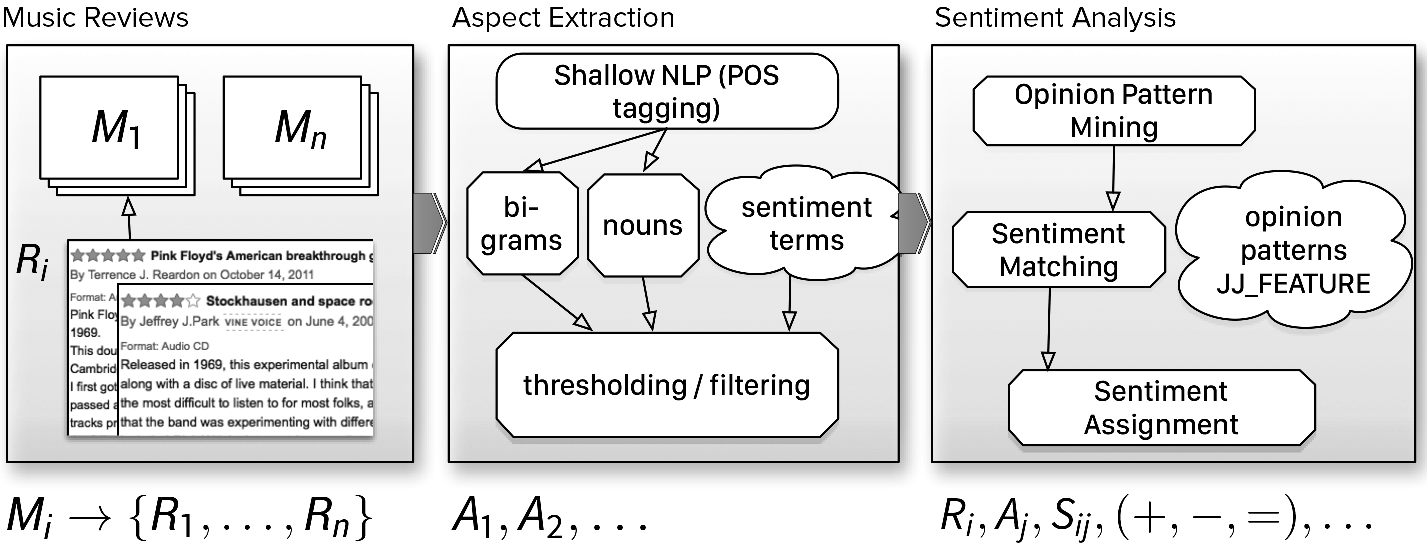
\includegraphics[width=\columnwidth]{ch05_musicology_pics/omf_bn.pdf}
\caption{Overview of the opinion mining and sentiment analysis framework.}
\label{fig:musicology:OMF}
\end{figure}

Following the work of \cite{DongSOS13,DongOS14} we use a combination of shallow NLP, opinion mining, and sentiment analysis to extract opinionated features from reviews. For reviews $R_{i}$ of each album, we mine bi-grams and single-noun aspects (or review features), see \cite{Hu2004}; e.g. bi-grams which conform to a noun followed by a noun (e.g. \emph{chorus arrangement}) or an adjective followed by a noun (e.g. \emph{original sound}) are considered, excluding bi-grams whose adjective is a sentiment word (e.g. \emph{excellent}, \emph{terrible}). Separately, single-noun aspects are validated by eliminating nouns that are rarely associated with sentiment words in reviews, since such nouns are unlikely to refer to item aspects. We refer to each of these extracted aspects $A_{j}$ as review aspects.

For a review aspect $A_{j}$ we determine if there are any sentiment words in the sentence containing $A_{j}$. If not, $A_{j}$ is marked neutral, otherwise we identify the sentiment word $w_{min}$ with the minimum word-distance to $A_j$. Next we determine the part-of-speach tags for $w_{min}$, $A_i$ and any words that occur between $w_{min}$ and $A_i$. 
%This POS sequence is an opinion pattern. We compute the frequency of all opinion patterns in all reviews; a pattern is valid if it occurs more than average. For valid patterns, we assign sentiment score between -1 and 1 to $A_j$ based on the sentiment of $w_{min}$ and subject to whether the corresponding sentence contains any negation terms within $4$ words of $w_{min}$. 
We assign a sentiment score between -1 and 1 to $A_j$ based on the sentiment of $w_{min}$, subject to whether the corresponding sentence contains any negation terms within $4$ words of $w_{min}$. If there are no negation terms, then the sentiment assigned to $A_j$ is that of the sentiment word in the sentiment lexicon; otherwise this sentiment is reversed. Our sentiment lexicon is derived from SentiWordNet \citep{esuli2006sentiwordnet} and is not specifically tuned for music reviews.
%If an opinion pattern is not valid then we assign a neutral sentiment to each of its occurrences within the review set; see \cite{Moghaddam2010} for a more detailed description. 
An overview of the process is shown in Figure~\ref{fig:musicology:OMF}. The end result of sentiment analysis is that we determine a sentiment label $S_{ij}$ for each aspect $A_j$ in review $R_i$. A sample annotated review is shown in Figure~\ref{fig:musicology:annotatedreview}.
Finally, the sentiment score of a review $R_i$ is calculated as the average of the sentiment score of every aspect $A_j$ in $R_i$.

\begin{figure}[h]
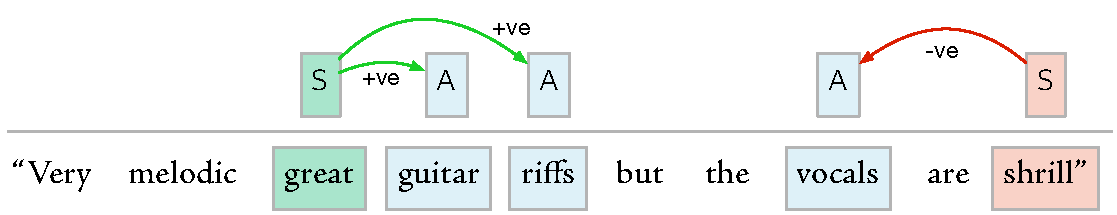
\includegraphics[width=\columnwidth]{ch05_musicology_pics/annotation_sample2}
\caption{A sentence from a sample review annotated with opinion and aspect pairs.}
\label{fig:musicology:annotatedreview}
\end{figure}

\subsection{Experiments}
\label{sec:musicology:experiments}

We carried out a study of the evolution of music criticism from two different temporal standpoints. Specifically, we consider when the review was written and, in addition, when the album was first published. We define the sentiment score of a review as the average score of all aspects in the review. Since we have sentiment information available for each review, we first computed an average sentiment score for each year of review publication (between 2000 and 2014). In this way, we may detect any significant fluctuation in the evolution of affective language during the 21st century. Then, we also calculated an average sentiment score by year of album publication. This information is complemented with the averages of the Amazon rating scores.

In what follows, we show visualizations for sentiment scores and correlation with ratings given by Amazon users, according to these two different temporal dimensions. Although arriving to musicological conclusions is out of the scope of this paper, we provide \textit{food for thought} and present the readers with hypotheses that may explain some of the facts revealed by these data-driven trends.

\begin{figure*}[ht!]
    \centering
    \begin{subfigure}{.32\textwidth}
        \centering
        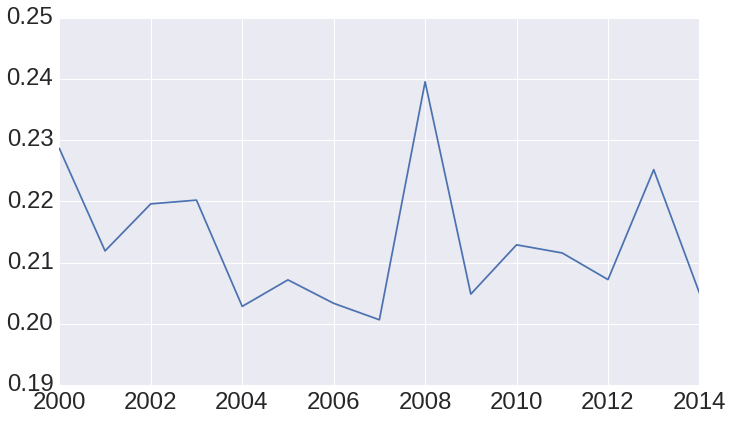
\includegraphics[width=.9\linewidth]{ch05_musicology_pics/all_average.png}
        \caption{Sentiment}
        \label{fig:musicology:avgSentReview}
    \end{subfigure}
    \begin{subfigure}{.32\textwidth}
        \centering
        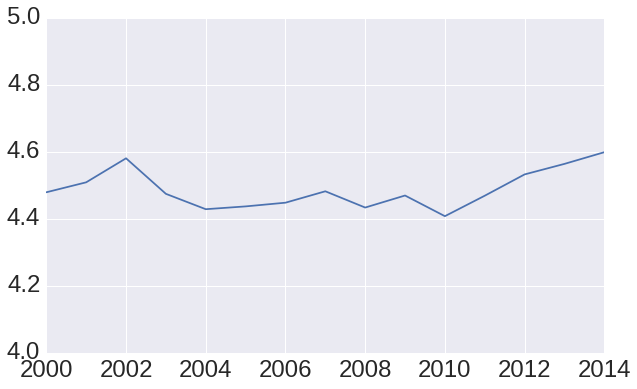
\includegraphics[width=.9\linewidth]{ch05_musicology_pics/avg_score.png}
        \caption{Rating}
        \label{fig:musicology:avgRatingReview}
    \end{subfigure}
    \begin{subfigure}{.32\textwidth}
        \centering
        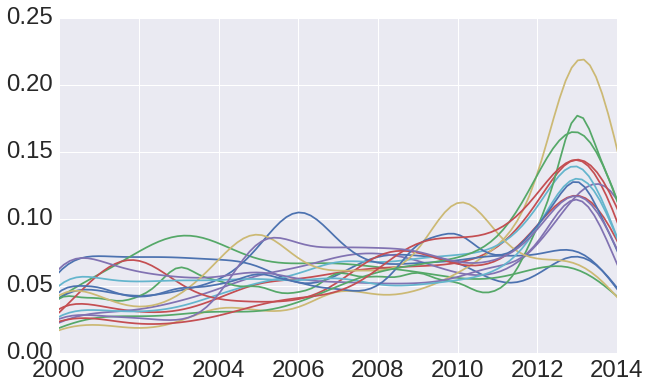
\includegraphics[width=.9\columnwidth]{ch05_musicology_pics/kde.png}
        \caption{Kernel density est.}
        \label{fig:musicology:kde}
    \end{subfigure}
    \begin{subfigure}{.32\textwidth}
        \centering
        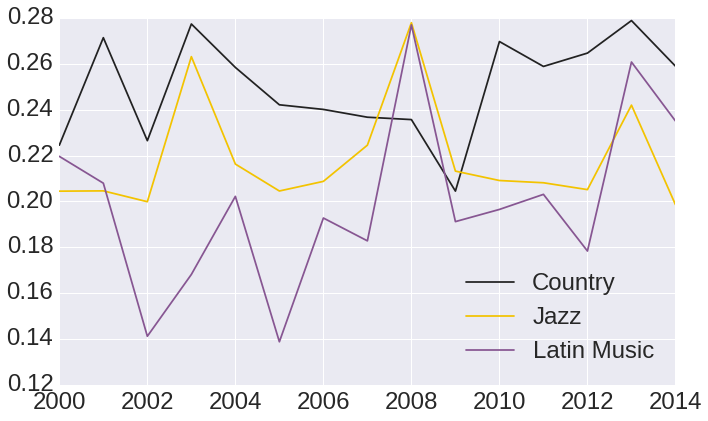
\includegraphics[width=.9\linewidth]{ch05_musicology_pics/genres_average.png}
        \caption{Sentiment by genre}
        \label{fig:musicology:avgSentReviewGenres}
    \end{subfigure}
    \begin{subfigure}{.32\textwidth}
        \centering
        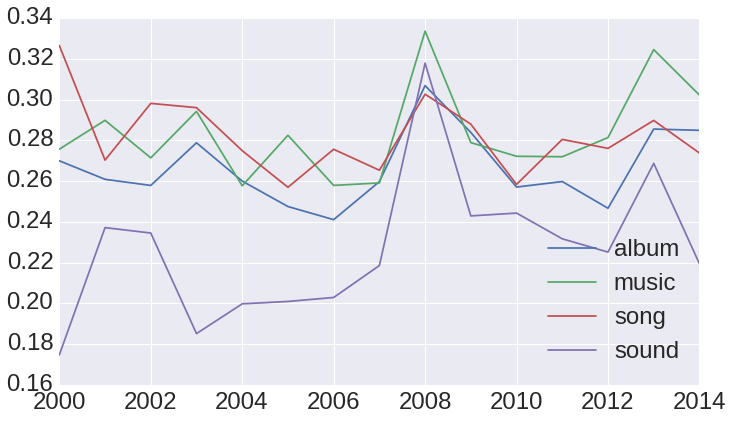
\includegraphics[width=.9\linewidth]{ch05_musicology_pics/main_aspects.png}
        \caption{Sentiment by aspect}
        \label{fig:musicology:avgSentReviewAspects}
    \end{subfigure}
    \begin{subfigure}{.32\textwidth}
        \centering
        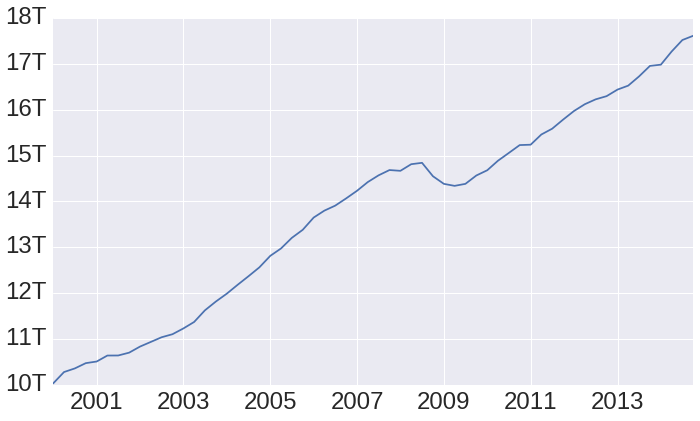
\includegraphics[width=.8\linewidth]{ch05_musicology_pics/gdp2.png}
        \caption{USA GDP trend}
        \label{fig:musicology:gdp}
    \end{subfigure}
 
   \begin{subfigure}{.32\textwidth}
        \centering
        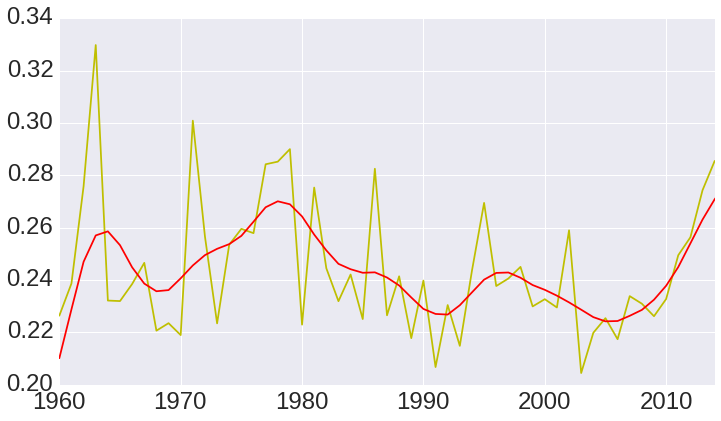
\includegraphics[width=.9\textwidth]{ch05_musicology_pics/sentiment_release_trend.png}
        \caption{Sentiment}
        \label{fig:musicology:avgSentimentRelease}
    \end{subfigure}
    \begin{subfigure}{.32\textwidth}
        \centering
        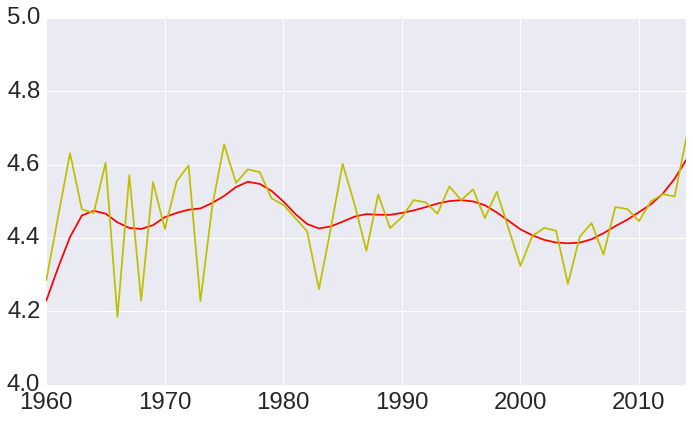
\includegraphics[width=.9\textwidth]{ch05_musicology_pics/rating_release_trend.png}
        \caption{Rating}
        \label{fig:musicology:avgRatingRelease}
    \end{subfigure}
    \begin{subfigure}{.32\textwidth}
        \centering
        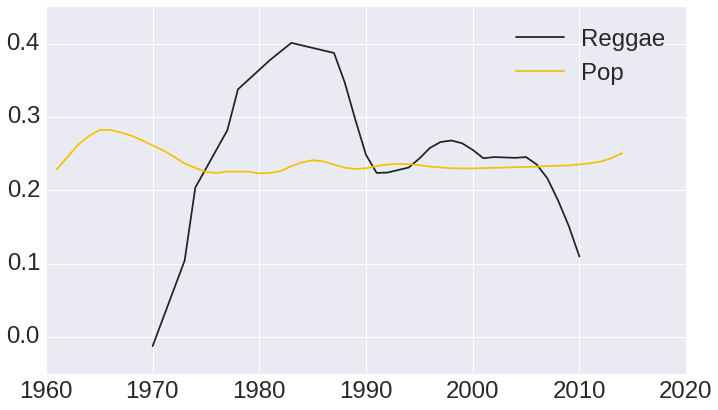
\includegraphics[width=.9\columnwidth]{ch05_musicology_pics/genres_release_trend.png}
        \caption{Sentiment by genre}
        \label{fig:musicology:avgSentimentGenresRelease}
    \end{subfigure}
    %\caption{Sentiment and rating averages by review publication year (a and b); GDP trend in USA from 2000 to 2014 (c), and sentiment and rating averages by album publication year (d, e and f)}
    \caption{Sentiment and rating averages by review publication year (a, b d and e); Kernel density estimation of the distribution of reviews by year (c); GDP trend in USA from 2000 to 2014 (f), and sentiment and rating averages by album publication year (g, h and i)}
\end{figure*}

\subsubsection{Evolution by review publication year}
\label{sec:musicology:evolution-review}

We applied sentiment and rating average calculations to the whole MARD dataset, grouping album reviews by year of publication of the review. Figure \ref{fig:musicology:avgSentReview} shows the average of the sentiment scores of all the reviews published in a specific year, whilst Figure~\ref{fig:musicology:avgRatingReview} shows average review ratings per year. At first sight, we do not observe any correlation between the trends illustrated in the figures. However, the sentiment curve (Figure~\ref{fig:musicology:avgSentReview}) shows a remarkable peak in 2008, a slightly lower one in 2013, and a low between 2003 and 2007, and also between 2009 and 2012. Figure~\ref{fig:musicology:kde} shows the kernel density estimation of the distribution of reviews by year of the 16 genres. The shape of these curves suggest that the 2008 peak in the sentiment score is not related to the number of reviews published that year. The peak persists if we construct the graphs with the average sentiment associated with the most repeated aspects in text (Figure \ref{fig:musicology:avgSentReviewAspects}). 
It is not trivial to give a proper explanation of this variations on the average sentiment. We speculate that these curve fluctuations may suggest some influence of economical or geopolitical circumstances in the language used in the reviews, such as the 2008 election of Barack Obama as president of the US. As stated by the political scientist Dominique Mo\"{i}si in \cite{Moisi2010}:

\begin{displayquote}\small{
In November 2008, at least for a time, hope prevailed over fear. The wall of racial prejudice fell as surely as the wall of oppression had fallen in Berlin twenty years earlier [...] Yet the emotional dimension of this election and the sense of pride it created in many Americans must not be underestimated.}
\end{displayquote}

If we calculate the sentiment evolution curve for the different genres (see Figure~\ref{fig:musicology:avgSentReviewGenres}), we observe that 2008 constitutes an all-time-high for almost all genres. It is remarkable that genres traditionally related to more diverse communities such as Jazz and Latin Music experience such an increase, whilst other genres such as Country do not.

Another factor that might be related to the positiveness in use of language is the economical situation. After several years of continuous economic growth, in 2007 a global economic crisis started\footnote{\url{https://research.stlouisfed.org}}, whose consequences were visible in the society after 2008 (see Figure~\ref{fig:musicology:gdp}). In any case, further study of the different implied variables is necessary to reinforce any of these hypotheses.

%Assuming that a vast majority of reviewers are North American (we do not have this information available), as the dataset was originally gathered from Amazon US, these trends may be explained with the 2008 election of president Barack Obama as president of the US. As stated by Dominique Mo\"{i}si in \cite{Moisi2010}:
%We assume that a vast majority of reviewers should be from the United States, as the dataset was originally gathered from the American version of the Amazon website.  
%Starting from this assumption, an important event happened in 2008 which affected not only United States citizens but the entire world, the election of Barak Obama as the President of the United Sates. As stated by Dominique Moïsi in \cite{Moisi2010}:



%Another factor that might be related to the positiveness in use of language is the economical situation. After several years of continuous economic growth, in 2007 a global economic crisis started, originated by the subprime mortgage crisis, whose consequences were more visible in the society from 2009 to 2013\footnote{\url{https://research.stlouisfed.org}}, as shown in Figure~\ref{fig:musicology:gdp}. %Following this hypothesis, the abrupt decrease of positiveness right after 2008 and its recovery by 2013 might be related to this. 
%In any case, further study of the different implied variables is necessary to reinforce any of these hypotheses.
    

%\begin{figure}
%    \centering
%    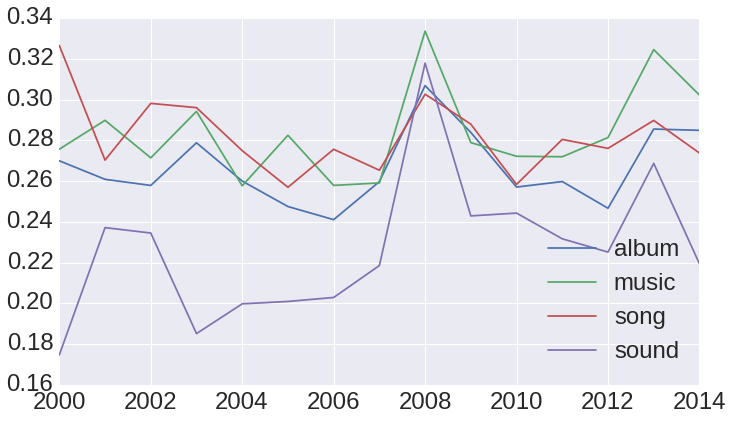
\includegraphics[width=.6\columnwidth]{ch05_musicology_pics/main_aspects.png}
%    \caption{Average sentiment of main aspects across genres by review year}
%    \label{fig:musicology:avgSentimentGenresReview}
%\end{figure}


\subsubsection{Evolution by album publication year}
\label{sec:musicology:evolution-album}

In this case, we study the evolution of the polarity of language by grouping reviews according to the album publication date. This date was gathered from MusicBrainz, meaning that this study is conducted on the ~42,1\% of the MARD that was successfully mapped. We compared again the evolution of the average sentiment polarity (Figure~\ref{fig:musicology:avgSentimentRelease}) with the evolution of the average rating (Figure~\ref{fig:musicology:avgRatingRelease}). Contrary to the results observed by review publication year, here we observe a strong correlation between ratings and sentiment polarity. To corroborate that, we computed first a smoothed version of the average graphs, by applying 1-D convolution (see line in red in Figures~\ref{fig:musicology:avgSentimentRelease} and \ref{fig:musicology:avgRatingRelease}). Then we computed Pearson's correlation between smoothed curves, obtaining a correlation $r = 0.75$, and a p-value $p \ll 0.001$. This means that in fact there is a strong correlation between the polarity identified by the sentiment analysis framework in the review texts, and the rating scores provided by the users. This correlation reinforces the conclusions that may be drawn from the sentiment analysis data. %, and reinforces the idea of averaging local sentiment scores as a measure of polarity in a review. %These sentiment scores might be used as an important feature for a rating prediction task.

To further dig into the utility of this polarity measure for studying genre evolution, we also computed the smoothed curve of the average sentiment by genre, and illustrate it with two idiosyncratic genres, namely \textit{Pop} and \textit{Reggae} (see  Figure~\ref{fig:musicology:avgSentimentGenresRelease}). We observe in the case of \textit{Reggae} that there is a time period where reviews have a substantial use of a more positive language between the second half of the 70s and the first half of the 80s, an epoch which is often called the golden age of \textit{Reggae} \citep{alleyne2012encyclopedia}. This might be related to the publication of Bob Marley albums, one of the most influential artists in this genre, and the worldwide spread popularity of reggae music. In the case of \textit{Pop}, we observe a more constant sentiment average. However, in the 60s and the beginning of 70s there are higher values, probably consequence by the release of albums by The Beatles. These results show that the use of sentiment analysis on music reviews over certain timelines may be useful to study genre evolution and identify influential events.


\section{Conclusions}
\label{sec:musicology:conclusions}

In this Chapter we have shown two different use cases in the context of making sense of large amounts of music related documents from a musicological perspective. (1) A culture-specific music knowledge base has been created, applying a process of automatic knowledge curation, which combines information coming from different data sources. In addition, the knowledge base has been enriched with content extracted directly from unstructured texts by using a custom entity linking system. A methodology to build knowledge graphs is described and tested for computing artist relevance ranking. Evaluation shows high correlation between the obtained ranking of artists and the opinion of a flamenco expert. 
%(2) an analysis on the evolution of Music Digital Libraries based on recent technology advancements have been reported. We pointed out that Music Digital Libraries are still in an early stage of development compared to latest developments on Web search. In addition, we proposed a methodology to exploit knowledge implicit in Digital Library documents, which has been applied on a corpus of artist biographies gathered from the New Grove Dictionary. 
(2) A diachronic study of the sentiment polarity expressed in customer reviews from two different standpoints has been presented. First, an analysis by year of review publication suggests that geopolitical events or macro-economical circumstances may influence the way people speak about music. Second, an analysis by year of album publication shows how sentiment analysis can be useful to study the evolution of music genres. Moreover, according to the observed trend curves, we can state that we are now in one of the happiest periods of the recent history of music. 

In conclusion, the main contribution of the work presented in this chapter is a demonstration of the utility of applying systematic linguistic processing on texts about music. Although further work is necessary to elaborate on the hypotheses or claims that may be derived from purely data-driven analyses, the proposed methodologies have shown their suitability in the quest of knowledge discovery from large amounts of documents, which may be highly useful for musicologists and humanities researchers in general.
